\documentclass{article}
\renewcommand{\familydefault}{\sfdefault}
\usepackage[a4paper, total={6in, 8in}]{geometry}
\usepackage{array}
\usepackage{graphicx}
\graphicspath{ {./images/} }

\title{Solid States}
\date{2021-04-17}
\author{Jeh}

\begin{document}
\maketitle
\pagenumbering{arabic}
   \section{One Mark Questions}
   \subsection{What are the types of particles in each of the main
   classes of crystalline solids?}

   \begin{itemize}
	\item Ionic Solids - \textbf{Cations and Anions}
	\item Covalent Network Solids - \textbf{Atoms}
	\item Molecular Solids - \textbf{Monoatomic and Polyatomic 
	Molecules}
	\item Metallic Solids - \textbf{Metallic ions in sea of 
	electron}
   \end{itemize}

   \subsection{Which of the three types of packing used by metals 
   makes the most efficient use of space and which makes the least
   efficient use of space?}

   Out of three types of packing fcc (or ccp or hcp) lattice makes the
   most efficient use of space while simple cubic lattice makes the 
   least efficient use of space.

   \subsection{What is the unit cell?}

   The smallest repeating structural unit of crystalline solid is
   called as unit cell of that solid.

   \subsection{How does the electrical conductivity of semiconductor
   changes with temperature? Why?}

   \begin{enumerate}
	\item The electrical conductivity of semiconductor increases
	with increasing temperature.
	\item This is because number of electrons with sufficient
	energy so as to get promoted to the conduction band increases
	as temperature rises. Thus, at higher temperatures, there are
	more mobile electrons in the conduction band and more 
	vacancies in the valence band than at lower temperature.
   \end{enumerate}

   \subsection{Solid is hard, brittle and electrically nonconductor.
   It melt conducts electrically. What type of solid is it?}

   Type of solid is - \textbf{Ionic Solid}

   \subsection{Mention two properties that are common to both hcp and
   ccp lattices. Give one property to both hcp and ccp crystal 
   lattices.}

   Properties common to both hcp and cpp lattice are the same
   coordination number \textbf{12} and the same parking efficiency 
   \textbf{74 percent}

   \section{2 and 3 Marks Question}
   \subsection{What are the valence band and conduction band?}
   
   \begin{enumerate}
	\item \textbf{Conduction Band -} \\ 
	The highest energy band formed by interactions of the outermost
	energy levels of closely spaced atoms in solids is called the
	conduction band.\\
	The conduction band may be partially occupied or vacant.
	Electrons in the conduction band are mobile and delocalized
	over the entire solid. They conduct electricity when an 
	electrical potential is applied.

	\item \textbf{Valence Band -}
	The bands having lower energy than conduction band is the
	valence band.\\
	The electrons in valence band are not free to move because
	they are tightly bound to respective nuclei.
   \end{enumerate}

   \subsection{Distinguish between ionic solids and molecular solids}

   \begin{center}
   \begin{tabular}{ | m{20em} | m{20em} | }
   \hline
   \textbf{Ionic Solids} & \textbf{Molecular Solids} \\
   \hline
   Charged ions (cations and anions & Monoatomic and polyatomic
   molecules \\
   \hline
   Held by electrostatic force of attraction between oppositely
   charged ions & Held by intermolecular forces of attractions 
   such as London forces, dipole-dipole forces and hydrogen force \\
   \hline
   Hard and Brittle & Soft \\
   \hline
   High melting points & Low Melting Points \\
   \hline
   Non-conductors of electricity in solid state. Good conductor when
   melted or dissolved in water & Poor conductors of electricity. \\
   \hline
   e.g. NaCl,etc. & Ice, Benzoic Acid, etc. \\
   \hline
   \end{tabular}
   \end{center}

   \subsection{How are the spheres arranged in first layer of simple
   cubic close-packed structures? How are the successive layers of
   spheres placed above this layer?}

   Simple cubic closed packed structures are obtained by stacking two-
   dimensional square close-packed layers.\\
   So, the spheres in the first layer are placed adjacent to one another
   to form the two dimensional square close packing (i.e.AAAA type
   arrangement). All the spheres of lower layers. This results in
   perfect horizontal and vertical alignment between the spheres of
   various layers.

   \subsection{What are the consequences of Schottky defect?}

   \textbf{Consequences of Schottky defect}
   \begin{enumerate}
	\item As the number of ions decreases, mass decreases. 
	However, the volume remains unchanged. Hence, the density of
	a substance decreases.
	\item The number of missing cations and anions is equal.
	Hence, the electrical neutrality of the compound is preserved.
   \end{enumerate}

   \subsection{How are the tetrahedral and octahedral voids formed?}

   \begin{enumerate}
	\item Two dimensional hexagonal close-packed layer has
	triangular voids which is formed by three spheres.
	\item When a triangular voids of the first layer are covered by
	spheres of the next layer, tetrahedral voids are formed.
	A tetrahedral voids are formed. A tetrahedral void is 
	surrounded by four spheres.
	\item The overlapping triangular voids from the two layers
	together form an octahedral void.\\
	An octahedral void is surrounded by six spheres.
   	\item Thus, the depression in which spheres of the second layer
	are tetrahedral voids while the depression in which no sphere
	rests are octahederal voids.\\\\
	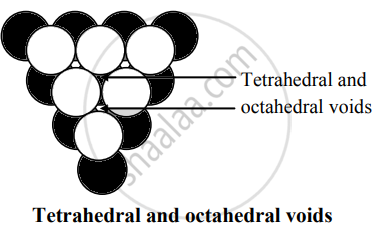
\includegraphics[scale=1.5]{voids}
   \end{enumerate}

   \subsection{Third layer of spheres is added to the second layer so
   as to form the hcp or ccp structure. What is the difference between
   the addition of the third layer to form these closed packed
   structures?}

   In cpp structure, the spheres of the third layer are not aligned
   with those of the first layer or second layer.\\
   Hence, the third is called as 'C' layer. The spheres of the fourth
   layer get aligned with the spheres of the first layer. Hence the
   fourth layer is called 'A' layer resulting in patterns of layer
   called 'ABCABC...'

   \subsection{Distinguish with the help of diagrams metal conductors,
   insulators and semiconductors from each other.}

   \begin{center}
   \begin{tabular}{ | m{15em} | m{15em} | m{15em} | }
   \hline
   \textbf{Metal Conductors} & \textbf{Insulators} &
   \textbf{Semiconductors}\\
   \hline
   Metals are good conductors of electricity & Insulators are
   conductors of electricity & Semiconductors have conductivity that
   is intermediate between conductors and insulators \\
   \hline
   In metal conductors, the conduction band is partially filled and
   there is no band gap or there is overlapping between the valence
   band or there is overlapping between valence band and conduction
   band & In insulators, the valence band and conduction band in 
   insulators are separated by large energy gap called forbidden 
   zone. & In semiconductors, the valence band is completely filled
   with electrons, and the conduction band is empty. However, the
   energy gap between the two bands is smaller than that in an
   insulator. \\
   \hline
   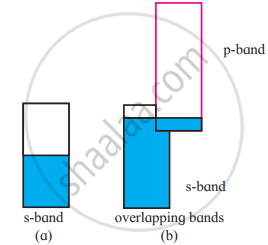
\includegraphics[scale=0.3]{metals}  &  
   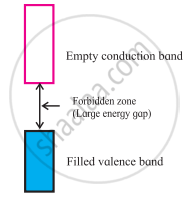
\includegraphics[scale=0.3]{insulators} &
   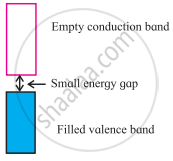
\includegraphics[scale=0.3]{semicon} \\
   \hline
   \end{tabular}
   \end{center}

   \subsection{What are the n-type semiconductors? Why is the
   conductivity of doped n-type semiconductor higher than that of pure
   semiconductor? Explain with diagram.}

   \begin{enumerate}
   \item An extrinsic semiconductor, which is obtained by adding group
   15 element to an intrinsic semiconductor which belongs to group 14,
   is called as n-type semiconductor.\\
   e.g Silicon doped with phosphorus.
   \item n-type semiconductor contains an increased number of electrons
   in the conduction band.
   \item Consider the doping of Si with phosphorus. Si has a crystal
   structure in which each Si atom is linked tetrahedrally to four
   other Si atoms. When a small quantity of phosphorus is added to
   pure Si, the P atoms occupy some vacant sites in the lattice in
   place of Si atoms. The overall crystal structure of Si remains
   unchanged. Four of the five valence electrons of P are utilized in
   bonding the closest to four Si atoms. Thus, P has one extra
   electron than needed for bonding. Therefore, Si doped with P has
   more number of electrons in the conduction band than those in
   conduction band in pure Si. Thus, the conductivity of Si-doped with
   P is higher than that of pure Si. The electrons of the conduction
   band move under the influence of an applied potential and conduct
   electricity.\\
   \end{enumerate}
   \textbf{P atom occupying regular site of Si atom}\\\\
   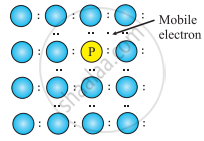
\includegraphics[scale=0.3]{mobile}
   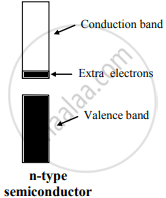
\includegraphics[scale=1.3]{ntype}

   \subsection{Explain with diagram, Frenkel defect. What are the
   conditions for its formation? What is its effects on density and
   electrical neutrality of the crystal?}

   \begin{itemize}
   \item \textbf{Frenkel defect:}
	 \begin{enumerate}
	 \item Frankel defect arises when an ion of an ionic compound is
	 missing from its regular lattice sites and occupies an
	 inters ilia position between lattice points. The cations are
	 usually smaller than anions. Therefore, the cations occupy
	 inters ilia sites.
	 \item The smaller cation is displaced from its normal site
	 to interstitial space. Therefore, it creates a vacancy defect
	 as it's original position and an interstitial defect at its
	 new location in the same crystal. Frenkel defect can regarded
	 as the combination of vacancy defect and interstitial defect.
	 \item This defect is found in ionic crystals like Zns, AgCl,
	 AgBr, Agl.
	 \end{enumerate}
   \textbf{Frenkel defect}\\
   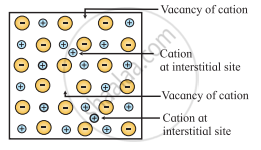
\includegraphics[scale=0.5]{frenkel}
   \item \textbf{Conditions for the formation of Frenkel Defect:}
	 \begin{enumerate}
	 \item Frenkel defect occurs in ionic compounds with large
	 difference between sizes of cation and anion.
	 \item The ions of ionic compounds must be having low
	 concentration number.
	 \end{enumerate}
   \item \textbf{Consequences of Frenke Defect:}
	 \begin{enumerate}
	 \item As no ions are missing from the crystal lattice as a
	 whole, the density of solid and its chemical properties remain
	 unchanged.
	 \item The crystal as a whole remains electrically neutral
	 because the equation numbers of cations and anions are
	 present.
	 \end{enumerate}
   \end{itemize}

   \subsection{What is the impurity defect? What are its types? Explain
   the formation of vacancies through aliovalent impurity with example.}

   \begin{enumerate}
   \item Impurity defect arises when a foreign atoms, that is atoms
   different from the host atoms, are present in the crystal lattice.
   \item There are two kinds of impurity defects : Substitutions and
   Interstitial impurity defects.
   \item Formation of vacancy through aliovalent impurity:\\
   Vacancies are created by the addition of the impurities of
   aliovalent ions (that is, ions with oxidation state different from
   host of ions) to an ionic solids.
   \end{enumerate}

   e.g. Consider a small amount of SrCl\textsuperscript{2} impurity
   added to NaCl during it crystallization. The added 
   Sr\textsuperscript{+2} ions (O.S. = +2) occupy some of the regular
   sites of Na\textsuperscript{+} host ions (O.S = +1). In order to
   maintain electrical neutrality, every Sr\textsuperscript{+2} ion
   removes two Na+ ions. One of the vacant lattice sites created by
   the removal of two Na\textsuperscript{+} ions is occupied by one
   Sr\textsuperscript{2+} ion. The other site of Na\textsuperscript{+}
   ion remains vacant as show in figure.\\\\

   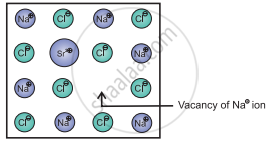
\includegraphics[scale=0.3]{vacan}
   

\end{document}
